\begin{frame}{RTDroid - Cross Context Channel}
	\only<2>{\centering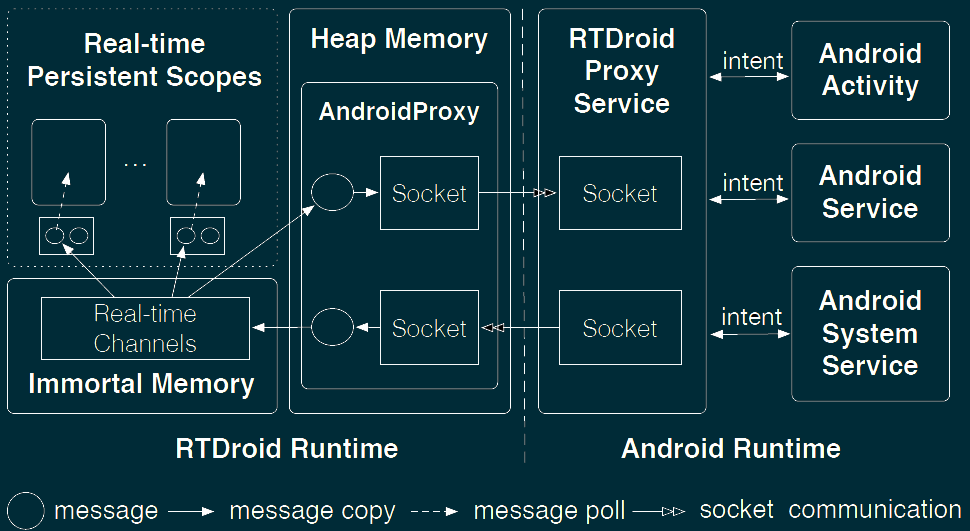
\includegraphics[scale=0.40]{crosscontext}}
	\only<1>{\begin{itemize}
		\item Permette di collegare due runtimes
		\item La comunicazione avviene tramite sockets
		\item I componenti non real-time non possono intasare la memoria dedicata a quelli real-time, perché i loro messaggi vengono salvati sullo heap
		\begin{itemize}
			\item Solo un messagio alla volta viene trasferito nella memoria immortal
		\end{itemize}
		\item Ai messaggi non real-time è assegnata la priorità più bassa, in modo da non generare interferenza
		\item In questo modo c'è la garanzia che la memoria non venga esaurita e che non vengano introdotti ritardi
	\end{itemize}}
\end{frame}